SyVOLT is a user-friendly Eclipse plugin to verify pre-/post- condition contracts on model transformations specified in the DSLTrans transformation language. The tool has a number of unique features, outlined below.

\subsection{Integration with Eclipse}

Providing our tool as an Eclipse plugin allows the user to work within a robust and popular development environment, while still allowing for easy setup of the prover. We are able to leverage the capabilities of Eclipse's graphical modelling evironments for artifact construction, as well as the Eclipse Generation Language (EGL) for the model-to-text production of required tool artifacts.

\subsection{Eclipse Frontend}

\begin{figure}
\centering
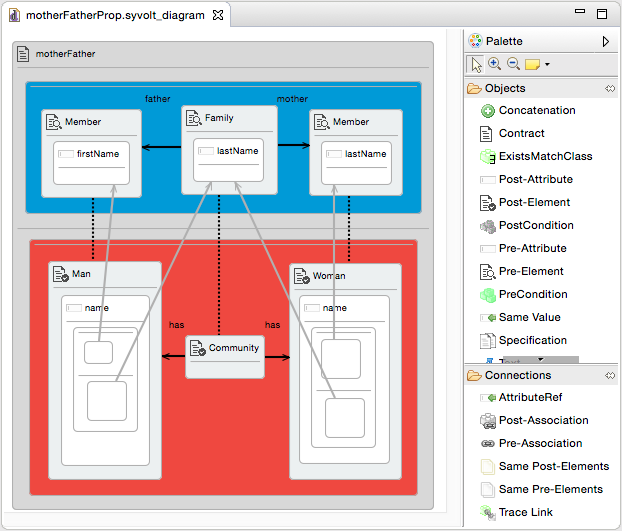
\includegraphics[width=0.45\textwidth]{figures/eclipse_frontend}
\caption{The transformation editor within Eclipse}
\label{fig:eclipse_frontend}
\end{figure}

Figure~\ref{fig:eclipse_frontend} shows the Eclipse frontend, where a user can edit a DSLTrans transformation within the Eclipse editor. A similar view is also used for users to define the contracts for their transformations. Note that these editors are based within the model creation framework FIX FIX.

\subsection{Graphical Modelling}
Both the transformation and the contracts are built using a graphical environment. This intuitive representation allows the user to quickly and easily visualize and construct the required contracts. This is in contrast to  the logical or mathematical expression approach which is required by other verification techniques.

\subsection{Import from ATL}
The Atlas Transformation Language (ATL) is commonly-used in both industry and academia applications. In order to extend our approach into these domains, we have developed a higher-order transformation that is able to automatically transform declarative ATL transformations into our transformation language DSLTrans~\cite{Oakes}. This allows the user to exhaustively prove contracts on ATL transformations.

\subsection{Handling of String Attributes}
The DSLTrans transformations and contracts are built upon typed graphs. 
Our contract prover is able to reason over these graphs to prove contracts. An example of this would be in the Families-To-Persons transformation from the ATL zoo [CITE]. In this transformation, the name for a person in the output graph is a concatenation of two strings from elements in the input graph. Our contract prover can prove that this concatenation will be valid in all cases.

\subsection{Push-Button Proving}
Once the transformation and the contracts of interest are created, one command will start the property proving process. This process will automatically create all required artifacts (as detailed in the following section), run the process, and then provide the results to the user within the Eclipse environment, as seen in Figure~\ref{fig:output}. This allows the user to continually stay within the Eclipse environment.

\begin{figure}
\centering
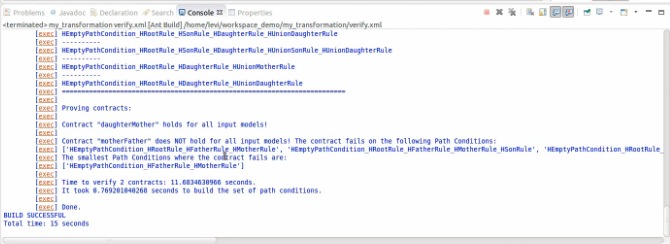
\includegraphics[width=0.45\textwidth]{figures/output}
\caption{The results of the contract prover}
\label{fig:output}
\end{figure}

\subsection{Input Independence and Exhaustiveness}

Our technique will exhaustively prove whether a contract will hold for all possible input models to a transformation. This allows us to exhaustively verify a transformation, as seen in~\cite{Lucio2014}.

\subsection{Proving Speed}

 Even though our technique is exhaustive, our approach takes a relatively short amount of time to prove contracts. For example, our experiments on industrial transformations~\cite{Oakes} show that contracts can be verified within a few minutes. \cite{Selim2014} demonstrates that our prover is faster than similar mathematical approaches.

\subsection{Production of Counter-Examples}

An advantage of our technique is that a counter-example model for a particular contract can be produced by the contract proving process. This allows the user to easily determine the error in the transformation and correct it. We suggest that this enables a transformation development method analogous to 'test-driven development'. In this method, development would be punctuated by contract proof in order to catch errors early.


\subsection{Model-Driven Development}

One principle of the Modelling, Design, and Simulation Lab is that all tools and processes should 

Everything is modelled. Model transformations, and tooling.
 